%%%%%%%%%%%%%%%%%%%%%%%%%%%%%%%%%%%%%%%%%%%%%%%%%%%%%%%%%%%%%%%%%%%%%%%%%%%%%%%
%                       CARGA DE LA CLASE DE DOCUMENTO                        %
%%%%%%%%%%%%%%%%%%%%%%%%%%%%%%%%%%%%%%%%%%%%%%%%%%%%%%%%%%%%%%%%%%%%%%%%%%%%%%%

\documentclass[11pt,spanish,listoffigures,listoftables]{tfgetsinf}

%%%%%%%%%%%%%%%%%%%%%%%%%%%%%%%%%%%%%%%%%%%%%%%%%%%%%%%%%%%%%%%%%%%%%%%%%%%%%%%
%                          CODIFICACIÓN DEL FICHERO                           %
%%%%%%%%%%%%%%%%%%%%%%%%%%%%%%%%%%%%%%%%%%%%%%%%%%%%%%%%%%%%%%%%%%%%%%%%%%%%%%%

\usepackage[utf8]{inputenc} 
\usepackage{babel}
\usepackage{hyperref}
\usepackage{biblatex}
\usepackage{amsmath, amssymb}
\usepackage{graphicx}
\usepackage{booktabs}
\usepackage{listings}
\usepackage{xcolor}
\usepackage{multirow}


\addbibresource{bib.bib}  % Enlazar el archivo .bib
\addglobalbib{bib.bib}
\hypersetup{ colorlinks=true, linkcolor=black, urlcolor=cyan }

%%%%%%%%%%%%%%%%%%%%%%%%%%%%%%%%%%%%%%%%%%%%%%%%%%%%%%%%%%%%%%%%%%%%%%%%%%%%%%%
%                             OTROS PAQUETES                                  %
%%%%%%%%%%%%%%%%%%%%%%%%%%%%%%%%%%%%%%%%%%%%%%%%%%%%%%%%%%%%%%%%%%%%%%%%%%%%%%%
% (Aquí puedes añadir los paquetes que necesites)

%%%%%%%%%%%%%%%%%%%%%%%%%%%%%%%%%%%%%%%%%%%%%%%%%%%%%%%%%%%%%%%%%%%%%%%%%%%%%%%
%                         DATOS DEL TRABAJO                                   %
%%%%%%%%%%%%%%%%%%%%%%%%%%%%%%%%%%%%%%%%%%%%%%%%%%%%%%%%%%%%%%%%%%%%%%%%%%%%%%%

\title{Uso de IA en la detección de Artrosis para rodillas}
\author{Hernández Martínez, Carlos}
\tutor{Juan Ciscar, Alfonso}
\curs{2024-2025}

%%%%%%%%%%%%%%%%%%%%%%%%%%%%%%%%%%%%%%%%%%%%%%%%%%%%%%%%%%%%%%%%%%%%%%%%%%%%%%%
%            PALABRAS CLAVE Y RESÚMENES (en tres idiomas)                     %
%%%%%%%%%%%%%%%%%%%%%%%%%%%%%%%%%%%%%%%%%%%%%%%%%%%%%%%%%%%%%%%%%%%%%%%%%%%%%%%

\keywords{Palabras clave en catalán} % catalán
         {Palabras clave en español} % español
         {Keywords in English}       % inglés

\begin{document}

%%%%%%%%%%%%%%%%%%%%%%%%%%%%%%%%%%%%%%%%%%%%%%%%%%%%%%%%%%%%%%%%%%%%%%%%%%%%%%%
%                             RESÚMENES                                       %
%%%%%%%%%%%%%%%%%%%%%%%%%%%%%%%%%%%%%%%%%%%%%%%%%%%%%%%%%%%%%%%%%%%%%%%%%%%%%%%

\begin{abstract}
Aquí citamos a un datajkjkset \cite{gornale2020digital}.
Citación paper IEE \cite{10863523}, Dataset \cite{chen2018knee}
aqui citamos un paper \cite{VAATTOVAARA2025100580}
otra cita \cite{comprehensive_review}

Quitar imagenes brillantes -> \cite{efficientnet_paper}
\end{abstract}

\begin{abstract}[spanish]
(Resumen en castellano)
\end{abstract}

\begin{abstract}[english]
(Resumen en inglés)
\end{abstract}

\mainmatter

%%%%%%%%%%%%%%%%%%%%%%%%%%%%%%%%%%%%%%%%%%%%%%%%%%%%%%%%%%%%%%%%%%%%%%%%%%%%%%%
%                              CAPÍTULO 1                                     %
%                                    INTRO                                     %
%%%%%%%%%%%%%%%%%%%%%%%%%%%%%%%%%%%%%%%%%%%%%%%%%%%%%%%%%%%%%%%%%%%%%%%%%%%%%%%

\chapter{Introducción}  % ~5 páginas

\section{Motivación}     % 1.1
La artritis es una de las enfermedades musculoesqueléticas más prevalentes a nivel mundial y una de las principales causas de discapacidad en adultos mayores. Su diagnóstico y seguimiento se basa tradicionalmente en la evaluación clínica y en la interpretación de imágenes médicas, como radiografías, resonancias magnéticas y tomografías computarizadas. Sin embargo, este proceso suele depender en gran medida de la experiencia del profesional médico, lo que puede generar variabilidad en los diagnósticos y retrasos en la detección temprana de la enfermedad.

En los últimos años, los avances en inteligencia artificial, y en particular en el aprendizaje profundo, han demostrado un gran potencial para mejorar la precisión y la eficiencia en el análisis de imágenes médicas. Las redes neuronales convolucionales (CNN) han sido ampliamente utilizadas en el campo de la visión por computadora para tareas como la detección de patologías en radiografías, la segmentación de tejidos en resonancias magnéticas y la clasificación de niveles de severidad en enfermedades degenerativas.

Este Trabajo de Fin de Grado (TFG) se motiva por la necesidad de desarrollar métodos automáticos y robustos para el análisis de la artritis mediante el uso de técnicas de aprendizaje profundo. En particular, se busca explorar el uso de redes neuronales para la clasificación de imágenes médicas, utilizando bases de datos estandarizadas como \textit{Mendeley dataset} \cite{chen2018knee}. La aplicación de estos modelos podría no solo optimizar el proceso de diagnóstico, sino también contribuir al desarrollo de herramientas de soporte a la decisión clínica, facilitando una intervención más temprana y personalizada para los pacientes.

La relevancia de este estudio radica en su potencial impacto en la práctica clínica. Un sistema basado en inteligencia artificial podría reducir la carga de trabajo de los especialistas, mejorar la objetividad del diagnóstico y ofrecer segundas opiniones automáticas que complementen la evaluación médica tradicional. Además, el desarrollo de estas tecnologías en el ámbito de la artritis podría sentar un precedente para su aplicación en otras enfermedades musculoesqueléticas, ampliando el alcance del aprendizaje profundo en el campo de la salud.

Además, se plantea la posibilidad de realizar \textit{transfer learning} utilizando modelos preentrenados en artritis humana para aplicarlos en el diagnóstico de artritis en gatos. Esta adaptación podría beneficiar la práctica veterinaria, proporcionando herramientas automatizadas para la evaluación de la enfermedad en animales y mejorando la precisión en su diagnóstico.

En este contexto, el presente trabajo busca contribuir al avance del uso de inteligencia artificial en la detección y análisis de la artritis, evaluando diferentes enfoques de redes neuronales y analizando su rendimiento en la clasificación de imágenes médicas. La motivación principal es demostrar la viabilidad y efectividad de estos modelos en un problema biomédico concreto, promoviendo la integración de tecnologías emergentes en el ámbito de la salud.


\section{Objetivos}      % 1.2
% Presenta aquí los 3 objetivos principales
% p.e. Objetivo 1, Objetivo 2, Objetivo 3

\section{Estructura del documento}  % 1.3
% Describe la organización de los capítulos y secciones

%%%%%%%%%%%%%%%%%%%%%%%%%%%%%%%%%%%%%%%%%%%%%%%%%%%%%%%%%%%%%%%%%%%%%%%%%%%%%%%
%                              CAPÍTULO 2                                     %
%                                PRELIMINARES                                 %
%%%%%%%%%%%%%%%%%%%%%%%%%%%%%%%%%%%%%%%%%%%%%%%%%%%%%%%%%%%%%%%%%%%%%%%%%%%%%%%

\chapter{Preliminares}  % ~15 páginas

\section{Aprendizaje automático}

El aprendizaje automático (\textit{Machine Learning, ML}) es una rama de la inteligencia artificial que se centra en el desarrollo de algoritmos y modelos capaces de aprender a partir de datos. Esta tecnología ha transformado múltiples disciplinas al permitir que los sistemas mejoren su desempeño en tareas específicas mediante la experiencia, sin requerir una programación explícita para cada situación. Desde sus orígenes en técnicas estadísticas básicas hasta los modernos enfoques de aprendizaje profundo, ML ha evolucionado significativamente, impulsado por el incremento en la disponibilidad de datos y el avance en capacidad computacional. 
% //IMAGEN: Gráfico histórico que ilustra la evolución de las técnicas de ML (desde métodos clásicos hasta deep learning).

En el análisis de imágenes médicas, el aprendizaje automático permite automatizar procesos críticos como la detección, clasificación y segmentación de patologías, lo que resulta en diagnósticos más rápidos y precisos. Por ejemplo, modelos basados en redes neuronales profundas han demostrado rendimientos comparables a los de expertos humanos en la identificación de anomalías en radiografías, resonancias magnéticas y tomografías computarizadas.
% //IMAGEN: Comparativa visual entre una imagen médica original y la detección de anomalías realizada por un modelo de ML.
\begin{figure}[htbp]
    \centering
    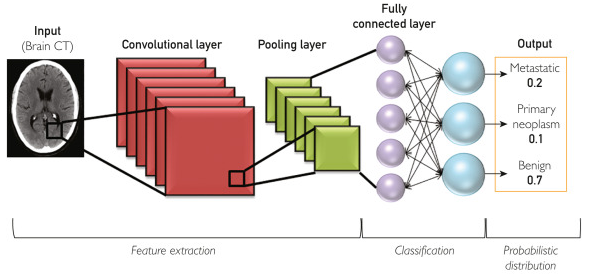
\includegraphics[width=1\textwidth]{neural_network.png}
    \caption{Descripción de la imagen}
    \label{fig:mi_imagen}
  \end{figure}
\subsection{Categorías de Aprendizaje Automático}

El aprendizaje automático se puede clasificar en tres paradigmas fundamentales:

\begin{itemize}
    \item \textbf{Aprendizaje supervisado}: Este enfoque utiliza conjuntos de datos etiquetados para entrenar modelos que aprendan a mapear entradas a salidas correctas. Algoritmos comunes en este paradigma incluyen la regresión lineal, las máquinas de soporte vectorial (SVM) y las redes neuronales profundas. 
    % //IMAGEN: Diagrama de flujo del proceso de aprendizaje supervisado.
    
    \item \textbf{Aprendizaje no supervisado}: En este caso, los datos no cuentan con etiquetas, y el objetivo es descubrir estructuras subyacentes o patrones en el conjunto de datos. Se emplean técnicas como el clustering, el análisis de componentes principales (PCA) y modelos generativos.
    % //IMAGEN: Ejemplo visual de un algoritmo de clustering aplicado a datos.
    
    \item \textbf{Aprendizaje por refuerzo}: Aquí, un agente interactúa con su entorno, tomando decisiones basadas en un sistema de recompensas y penalizaciones. A través de la retroalimentación, el agente aprende a optimizar su comportamiento para maximizar la función de recompensa.
    % //IMAGEN: Esquema que muestra el ciclo de interacción en el aprendizaje por refuerzo.
\end{itemize}

\subsection{Procesamiento de Datos en Aprendizaje Automático}

La calidad de los datos de entrada es determinante para el rendimiento y la capacidad de generalización de un modelo de ML. Por ello, el procesamiento de datos abarca varias fases esenciales:

\begin{itemize}
    \item \textbf{Preprocesamiento}: Consiste en la limpieza, normalización y transformación de los datos para eliminar ruidos y gestionar valores faltantes. En el caso de imágenes médicas, este proceso puede incluir la corrección de artefactos, la estandarización de intensidades y la segmentación preliminar de regiones de interés.
    % //IMAGEN: Diagrama que ilustra el flujo de preprocesamiento en imágenes médicas.
    
    \item \textbf{División del conjunto de datos}: Se segmenta la información en subconjuntos de entrenamiento, validación y prueba. Esta división es crucial para ajustar los hiperparámetros del modelo, prevenir el sobreajuste y evaluar de forma objetiva el desempeño final.
    % //IMAGEN: Representación gráfica de la partición de datos en entrenamiento, validación y test.
    
    \item \textbf{Extracción y selección de características}: En algunos casos, es necesario identificar y extraer características relevantes que potencien la capacidad del modelo para detectar patrones significativos, especialmente en dominios de alta dimensionalidad.
\end{itemize}

\subsection{Métricas de Evaluación}

La evaluación del rendimiento de los modelos de aprendizaje automático se realiza mediante diversas métricas, que varían según la naturaleza del problema:

\begin{itemize}
    \item \textbf{Para clasificación}: Se utilizan métricas como la precisión (\textit{accuracy}), la precisión (precision), la sensibilidad (recall) y el F1-score. La curva ROC y el área bajo la curva (AUC-ROC) también son fundamentales para evaluar la capacidad del modelo para distinguir entre clases.
    % //IMAGEN: Ejemplo gráfico de una curva ROC con el cálculo del AUC.
    
    \item \textbf{Para regresión}: Se emplean métricas como el error cuadrático medio (MSE) y el error absoluto medio (MAE), que cuantifican la diferencia entre las predicciones y los valores reales.
\end{itemize}

\subsection{Aplicaciones del Aprendizaje Automático en Imágenes Médicas}

La integración de ML en el análisis de imágenes médicas ha permitido avances significativos en el campo del diagnóstico y la intervención clínica. Entre las aplicaciones más relevantes se encuentran:

\begin{itemize}
    \item \textbf{Detección de enfermedades}: Modelos supervisados permiten identificar anomalías en diversos tipos de imágenes médicas, facilitando diagnósticos tempranos y precisos.
    % //IMAGEN: Ejemplo de radiografía con áreas destacadas que indican anomalías.
    
    \item \textbf{Segmentación de tejidos y órganos}: Las redes neuronales, especialmente las CNN, posibilitan la delimitación precisa de regiones de interés, lo cual es esencial para planificar tratamientos y procedimientos quirúrgicos.
    % //IMAGEN: Imagen segmentada de una resonancia magnética mostrando la delimitación de órganos.
    
    \item \textbf{Clasificación de tumores}: Los modelos de aprendizaje profundo pueden diferenciar entre tumores benignos y malignos, proporcionando una segunda opinión automatizada que complementa la evaluación clínica.
\end{itemize}

\subsection{Ventajas, Desafíos y Perspectivas Futuras}

El aprendizaje automático ofrece múltiples ventajas en el ámbito médico, aunque también presenta desafíos que requieren atención:

\begin{itemize}
    \item \textbf{Ventajas}:
    \begin{itemize}
        \item Automatización del análisis de grandes volúmenes de datos.
        \item Capacidad para detectar patrones complejos y no lineales.
        \item Reducción de la variabilidad interobservador en el diagnóstico.
    \end{itemize}
    % //IMAGEN: Tabla comparativa de las ventajas del aprendizaje automático en imágenes médicas.
    
    \item \textbf{Desafíos}:
    \begin{itemize}
        \item La necesidad de contar con grandes volúmenes de datos etiquetados.
        \item Riesgo de sobreajuste y la necesidad de aplicar técnicas de regularización.
        \item Problemas de interpretabilidad, lo que puede dificultar la adopción en entornos clínicos.
    \end{itemize}
    % //IMAGEN: Diagrama que ilustra los desafíos del sobreajuste y la interpretabilidad en ML.
    
    \item \textbf{Perspectivas Futuras}:
    La investigación en ML continúa avanzando hacia modelos más robustos y explicables. El desarrollo de técnicas de transferencia de aprendizaje, la integración de algoritmos híbridos y el fomento de la interpretabilidad serán clave para una mayor adopción en el ámbito médico, permitiendo sistemas de apoyo al diagnóstico cada vez más precisos y confiables.
    % //IMAGEN: Esquema que presenta las tendencias futuras en el desarrollo de ML para aplicaciones médicas.
\end{itemize}

En resumen, el aprendizaje automático representa una herramienta poderosa que, a través de su continua evolución, promete revolucionar el análisis de imágenes médicas. Su capacidad para automatizar y mejorar procesos diagnósticos no solo optimiza la eficiencia clínica, sino que también abre la puerta a un futuro en el que la inteligencia artificial se integre de manera efectiva en la toma de decisiones médicas.


\section{Redes neuronales}
Las redes neuronales son modelos computacionales inspirados en el funcionamiento del cerebro humano, diseñados para reconocer patrones y aprender representaciones a partir de datos. Su capacidad para aproximar funciones complejas las ha convertido en una herramienta fundamental en el ámbito del aprendizaje profundo y el análisis de imágenes médicas.

\subsection{Estructura y Funcionamiento}
Una red neuronal se compone de varias capas de neuronas artificiales:
\begin{itemize}
    \item \textbf{Capa de entrada:} Recibe los datos iniciales y los distribuye a las neuronas de las capas siguientes.
    \item \textbf{Capas ocultas:} Una o varias capas intermedias que transforman las entradas mediante combinaciones lineales y funciones de activación no lineales, permitiendo la extracción de características relevantes.
    \item \textbf{Capa de salida:} Genera la respuesta final del modelo, que puede corresponder a una clasificación, una regresión u otra tarea específica.
\end{itemize}
Cada neurona realiza una suma ponderada de sus entradas, seguida de la aplicación de una función de activación (por ejemplo, sigmoide, ReLU o tanh), lo que introduce la no linealidad necesaria para modelar relaciones complejas.

\subsection{Proceso de Aprendizaje y Optimización}
El aprendizaje en redes neuronales se basa en la minimización de una función de coste, que cuantifica la diferencia entre las predicciones del modelo y los valores reales. Este proceso se lleva a cabo mediante:
\begin{itemize}
    \item \textbf{Backproping:} Algoritmo que permite calcular el gradiente del error con respecto a cada peso en la red, facilitando su ajuste.
    \item \textbf{Descenso de gradiente:} Método de optimización utilizado para actualizar los pesos de forma iterativa y reducir la función de coste.
\end{itemize}
El éxito del aprendizaje depende, en gran medida, de la elección de la función de activación, la arquitectura de la red y los hiperparámetros del algoritmo de optimización.

\subsection{Principales Arquitecturas de Redes Neuronales}
Existen diversas configuraciones de redes neuronales, cada una adaptada a distintos tipos de problemas:
\begin{itemize}
    \item \textbf{Redes Feedforward:} La información fluye en una única dirección desde la entrada hasta la salida, siendo las más simples en estructura.
    \item \textbf{Redes Convolucionales (CNN):} Especializadas en el procesamiento de datos con estructura de grilla, como imágenes. Su uso es fundamental en tareas de visión por computadora, donde permiten extraer características espaciales relevantes.
    \item \textbf{Redes Recurrentes (RNN):} Diseñadas para trabajar con datos secuenciales, en las que la información de estados anteriores influye en las predicciones actuales.
\end{itemize}

\subsection{Aplicaciones en Imágenes Médicas}
En el análisis de imágenes médicas, las redes neuronales, y en particular las CNN, han demostrado un alto rendimiento en tareas como:
\begin{itemize}
    \item \textbf{Detección de anomalías:} Identificación de patrones sutiles en radiografías, resonancias magnéticas y tomografías computarizadas.
    \item \textbf{Clasificación de tejidos y tumores:} Diferenciación entre estructuras normales y patológicas, lo que contribuye a diagnósticos tempranos y precisos.
    \item \textbf{Segmentación de imágenes:} Delimitación precisa de regiones de interés, facilitando la planificación de tratamientos y procedimientos quirúrgicos.
\end{itemize}

\subsection{Desafíos y Perspectivas Futuras}
A pesar de su éxito, el uso de redes neuronales enfrenta desafíos importantes:
\begin{itemize}
    \item \textbf{Sobreajuste:} La tendencia del modelo a aprender de memoria los datos de entrenamiento, lo que afecta su capacidad de generalización.
    \item \textbf{Necesidad de grandes volúmenes de datos:} La obtención de conjuntos de datos suficientemente amplios y representativos es crucial para el entrenamiento eficaz.
    \item \textbf{Interpretabilidad:} La complejidad de los modelos dificulta la comprensión de las decisiones tomadas, lo que puede limitar su adopción en entornos clínicos.
\end{itemize}
La investigación continúa en áreas como la regularización, el aprendizaje por transferencia y los modelos interpretables, lo que promete mejorar la robustez y aplicabilidad de las redes neuronales en el ámbito médico.



\section{ML aplicado a CV y tareas biomédicas (MedMNIST)}
El uso de técnicas de Machine Learning (ML) en visión por computadora (CV) ha revolucionado el análisis de imágenes, permitiendo automatizar tareas que antes requerían la intervención humana directa. En el ámbito biomédico, estas técnicas han facilitado el diagnóstico y seguimiento de diversas patologías mediante la extracción de información relevante de imágenes médicas.

\subsection{Aplicaciones de ML en Visión por Computadora}
Las principales aplicaciones de ML en CV incluyen:
\begin{itemize}
    \item \textbf{Clasificación:} Consiste en asignar a cada imagen una etiqueta o categoría, aprovechando la capacidad de las redes neuronales para aprender características discriminativas de forma automática.
    \item \textbf{Detección de Objetos:} Permite localizar y etiquetar instancias específicas dentro de una imagen, lo cual es crucial para identificar estructuras anatómicas o anomalías.
    \item \textbf{Segmentación:} Divide una imagen en regiones o segmentos homogéneos, facilitando la delimitación de órganos o zonas afectadas, y ofreciendo un soporte esencial para diagnósticos precisos.
\end{itemize}
Estas técnicas se basan principalmente en arquitecturas de redes neuronales convolucionales (CNN), que han demostrado un desempeño sobresaliente en el procesamiento de imágenes.

\subsection{MedMNIST: Un Benchmark para Imágenes Médicas}
MedMNIST es un conjunto de datos diseñado específicamente para evaluar modelos de ML en tareas de clasificación de imágenes médicas. Entre sus características destacan:
\begin{itemize}
    \item \textbf{Diversidad de Modalidades:} Incluye imágenes provenientes de distintas modalidades médicas, como radiografías, resonancias magnéticas y tomografías computarizadas, lo que permite evaluar la versatilidad de los modelos.
    \item \textbf{Baja Resolución:} Las imágenes en MedMNIST tienen resoluciones relativamente bajas, simulando escenarios donde la disponibilidad de datos de alta calidad es limitada y exigiendo modelos robustos y eficientes.
    \item \textbf{Estándares de Evaluación:} El benchmark define protocolos de evaluación homogéneos, facilitando la comparación objetiva del desempeño de distintos algoritmos de ML.
\end{itemize}
El uso de MedMNIST permite a la comunidad investigadora explorar nuevas arquitecturas y técnicas de preprocesamiento, fomentando el desarrollo de modelos más adaptados a las condiciones reales del entorno biomédico.

\subsection{Integración de ML en Proyectos Biomédicos}
La aplicación de ML en proyectos biomédicos mediante técnicas de visión por computadora implica varios pasos:
\begin{itemize}
    \item \textbf{Preprocesamiento de Imágenes:} Involucra la normalización, corrección de artefactos y, en algunos casos, la segmentación preliminar para mejorar la calidad de las imágenes antes del análisis.
    \item \textbf{Diseño de Arquitecturas CNN:} Se desarrollan modelos específicos que aprovechan el aprendizaje transferido y técnicas de data augmentation para contrarrestar la limitación en la cantidad de datos disponibles.
    \item \textbf{Evaluación y Validación:} Se utilizan métricas especializadas, como la precisión, la sensibilidad, la especificidad y el AUC-ROC, para asegurar que el modelo sea robusto y fiable en contextos clínicos.
\end{itemize}
La integración de estas técnicas en sistemas de apoyo al diagnóstico contribuye a reducir la variabilidad interobservador y mejora la eficiencia en la detección temprana de patologías.

En conclusión, la combinación de ML y CV ha abierto nuevas posibilidades en el análisis de imágenes médicas. MedMNIST se erige como una herramienta fundamental para la validación y comparación de algoritmos, impulsando la innovación en el desarrollo de soluciones que pueden transformar el proceso diagnóstico en entornos clínicos.


%%%%%%%%%%%%%%%%%%%%%%%%%%%%%%%%%%%%%%%%%%%%%%%%%%%%%%%%%%%%%%%%%%%%%%%%%%%%%%%
%                              CAPÍTULO 3                                     %
%                      PRIMERA CONTRIBUCIÓN (OBJETIVO 1)                      %
%%%%%%%%%%%%%%%%%%%%%%%%%%%%%%%%%%%%%%%%%%%%%%%%%%%%%%%%%%%%%%%%%%%%%%%%%%%%%%%

\chapter{Capítulo 1 de contribución}  % ~15 páginas

El objetivo principal de este capítulo es replicar y ampliar el estudio realizado en \cite{10863523} aplicando técnicas avanzadas de aprendizaje profundo al análisis de imágenes de rodillas, utilizando el conjunto de datos proporcionado en \cite{chen2018knee}. La detección temprana de artrosis resulta crucial para la intervención clínica oportuna, y la automatización del proceso diagnóstico mediante inteligencia artificial ofrece una solución prometedora para reducir la variabilidad en la interpretación de imágenes médicas y aliviar la carga de trabajo en los centros de salud.

La elección de utilizar el modelo \textbf{EfficientNetB5} se fundamenta en su reconocido equilibrio entre precisión y eficiencia computacional. Su capacidad para aprender representaciones complejas a partir de imágenes médicas lo convierte en un candidato ideal para abordar los retos inherentes a la clasificación de patologías en rodillas. Además, la replicación del estudio original permite validar la reproducibilidad de los resultados y sienta las bases para futuras investigaciones y mejoras en la metodología.

\section{Metodología y Adaptaciones del Modelo}
Para la replicación del estudio, se parte de un modelo preentrenado de \textbf{EfficientNetB5} que se ha adaptado para ajustarse al problema específico de la detección de artrosis en imágenes de rodilla. La principal modificación realizada consiste en la redefinición de la capa de clasificación, adaptándola para discriminar entre las cinco clases presentes en el dataset. La nueva arquitectura de la capa de clasificación es la siguiente:

\begin{verbatim}
self.efficientnet.classifier = nn.Sequential(
    nn.Linear(in_features, 256),
    nn.ReLU(),
    nn.Linear(256, 256),
    nn.ReLU(),
    nn.Linear(256, num_classes),
    nn.Softmax(dim=1)
)
\end{verbatim}

Esta estructura permite transformar las características extraídas por la red en probabilidades asociadas a cada clase, facilitando una toma de decisiones más precisa durante el proceso de clasificación.

\section{Configuración del Entrenamiento y Optimización}
El proceso de entrenamiento del modelo se ha diseñado cuidadosamente para garantizar la robustez y la capacidad de generalización del sistema. Se ha empleado la función de pérdida \textbf{CrossEntropy}, idónea para problemas de clasificación múltiple, complementada con técnicas de regularización que combinan penalizaciones L1 y L2 (coeficiente de 0.001) para mitigar el riesgo de sobreajuste.

Los hiperparámetros críticos definidos para el entrenamiento son los siguientes:
\begin{itemize}
    \item \textbf{Paciencia} (*patience*): 5
    \item \textbf{Factor de reducción del learning rate} (*factor*): 0.1
    \item \textbf{Tasa de aprendizaje inicial} (*lr*): 0.001
    \item \textbf{Betas}: (0.9, 0.999)
\end{itemize}

Para la optimización se ha optado por el algoritmo \textbf{Adam}, reconocido por su adaptabilidad en entornos con datos complejos, mientras que el ajuste dinámico de la tasa de aprendizaje se realiza mediante el scheduler \textbf{ReduceLROnPlateau}. Este enfoque permite ajustar la tasa de aprendizaje en función de la evolución de la función de pérdida, contribuyendo a una convergencia más estable y eficiente:

\begin{verbatim}
optimizer = torch.optim.Adam(self.model.parameters(),
                             lr=self.learning_rate,
                             betas=self.betas)

scheduler = torch.optim.lr_scheduler.ReduceLROnPlateau(optimizer=optimizer,
                                                       factor=self.factor,
                                                       patience=self.patience)
\end{verbatim}

\section{Preprocesamiento y Aumento de Datos}
El conjunto de datos empleado, conocido como \textit{Mendeley dataset}\cite{gornale2020digital}, se ha dividido en subconjuntos de entrenamiento (70\%), test (20\%) y validación (10\%), asegurando una adecuada representación de cada clase. Para potenciar la capacidad del modelo y mejorar su generalización, se ha aplicado una serie de técnicas de aumento de datos utilizando transformaciones aleatorias. Estas transformaciones incluyen:
\begin{itemize}
    \item Rotación de imágenes hasta 20 grados.
    \item Desplazamientos horizontales y verticales de hasta un 20\% del tamaño de la imagen.
    \item Aplicación de cizallamiento (shear) y zoom.
    \item Inversión horizontal aleatoria.
\end{itemize}

El proceso de aumento de datos ha permitido transformar un conjunto original con distribución desequilibrada en un dataset equilibrado, alcanzando aproximadamente 1000 muestras por clase en el conjunto de entrenamiento. La distribución de imágenes es la siguiente:

\begin{center}
\begin{tabular}{lccccc}
\textbf{Clase} & 0 & 1 & 2 & 3 & 4 \\
\hline
\textbf{Train (original)} & 359 & 333 & 162 & 154 & 144 \\
\textbf{Validation} & 51 & 47 & 23 & 22 & 20 \\
\textbf{Test} & 104 & 97 & 47 & 45 & 42 \\
\hline
\textbf{Train (aumentado)} & 1000 & 1000 & 1000 & 1000 & 1000 \\
\end{tabular}
\end{center}

\section{Implementación del Modelo en PyTorch}
La implementación se ha desarrollado en PyTorch, lo que ha permitido una integración eficiente de módulos preentrenados y una configuración flexible para la experimentación. A modo de ejemplo, se presenta una versión simplificada de la clase \texttt{EfficientNetB5Custom}, que incorpora las modificaciones descritas:

\begin{verbatim}
class EfficientNetB5Custom(nn.Module):
    def __init__(self, num_classes=5, pretrained=True):
        super(EfficientNetB5Custom, self).__init__()
        if pretrained:
            self.efficientnet = models.efficientnet_b5(weights=EfficientNet_B5_Weights.DEFAULT)
        else:
            self.efficientnet = models.efficientnet_b5(weights=None)
        self.name = "EfficientNetB5Custom"
        in_features = self.efficientnet.classifier[1].in_features
        self.efficientnet.classifier = nn.Sequential(
            nn.Linear(in_features, 256),
            nn.ReLU(),
            nn.Linear(256, 256),
            nn.ReLU(),
            nn.Linear(256, num_classes),
            nn.Softmax(dim=1)
        )
    
    def forward(self, x):
        return self.efficientnet(x)
\end{verbatim}

Paralelamente, se ha definido un pipeline de preprocesamiento para las imágenes mediante las siguientes transformaciones:

\begin{verbatim}
transform = transforms.Compose([
    transforms.Resize((224, 224)),
    transforms.ToTensor(),
    transforms.Normalize(mean=[0.485, 0.456, 0.406], 
                         std=[0.229, 0.224, 0.225]),
])
\end{verbatim}

La configuración de entrenamiento adicional se ha establecido con los siguientes parámetros:
\begin{itemize}
    \item \textbf{BATCH\_SIZE}: 20
    \item \textbf{LEARNING\_RATE}: 0.001
    \item \textbf{FACTOR}: 0.001
    \item \textbf{Regularización L1}: 0.0001
    \item \textbf{Regularización L2}: 0.0001
    \item \textbf{PATIENCE}: 5
    \item \textbf{BETAS}: (0.9, 0.999)
\end{itemize}

\section{Resultados y Discusión}
Tras el entrenamiento, se obtuvieron los siguientes resultados en el conjunto de prueba:
\begin{itemize}
    \item \textbf{Loss}: 1.16
    \item \textbf{Accuracy (ACC)}: 0.74
    \item \textbf{Área bajo la curva (AUC)}: 0.92
\end{itemize}

La \textbf{Matriz de Confusión} para las cinco clases (0 a 4) se muestra a continuación:

\begin{table}[h]
\centering
\begin{tabular}{cc|ccccc}
    & \multicolumn{1}{c}{} & \multicolumn{5}{c}{\textbf{Predicción}} \\ 
    & \multicolumn{1}{c}{} & 0 & 1 & 2 & 3 & 4 \\ \cline{3-7}
\multirow{5}{*}{\textbf{Clase Real}}    
& 0 & 44 & 4  & 3 & 0  & 0 \\
& 1 & 5  & 36 & 6 & 0  & 0 \\
& 2 & 3  & 11 & 6 & 3  & 0 \\
& 3 & 0  & 3  & 2 & 17 & 0 \\
& 4 & 0  & 2  & 1 & 0  & 17 \\
\end{tabular}
\caption{Matriz de confusión del modelo \textit{EfficientNetB5Custom} en el conjunto de prueba.}
\end{table}

Precision = TP/(TP+FP) \\
Sensibilidad (Recall) = TP/(TP+FN) \\
Especificidad = TN/(TN+FP) \\
F1 = 2 * (Precision * Recall) / (Precision + Recall) \\

\begin{table}[h]
\centering
\begin{tabular}{c|cccc}
\hline
\textbf{Clase} & \textbf{Precisión} & \textbf{Sensibilidad} & \textbf{Especificidad} & \textbf{F1} \\
\hline
0 & 0.8461 & 0.8627 & 0.9285 & 0.8543 \\
1 & 0.7058 & 0.7659 & 0.8275 & 0.6990 \\
2 & 0.3333 & 0.2608 & 0.9140 & 0.2926 \\
3 & 0.8500 & 0.7727 & 0.9787 & 0.8095 \\
4 & 1.0000 & 0.8500 & 1.0000 & 0.9189 \\
\hline
\end{tabular}
\caption{Métricas de evaluación por clase en el conjunto de prueba.}
\label{tab:metricas-clase}
\end{table}

En ella se aprecia un desempeño satisfactorio en la mayoría de las clases, con especial eficacia para las clases 0 y 4. Sin embargo, existe cierta confusión entre las clases 1 y 2, lo que sugiere la necesidad de refinar la estrategia de preprocesamiento o ajustar hiperparámetros que permitan una mejor discriminación en futuros experimentos.

La precisión global (0.74) y el \textit{AUC} (0.92) indican que, a pesar de los falsos positivos y negativos observados, el modelo presenta una capacidad notable para distinguir entre diferentes niveles de artrosis. Con todo, se prevén mejoras adicionales si se profundiza en técnicas de regularización o se evalúan arquitecturas alternativas de redes neuronales.

\section{Conclusión del Capítulo}
En este capítulo se ha descrito el proceso de replicación del estudio de \cite{10863523} con un modelo \textbf{EfficientNetB5} adaptado al diagnóstico de artrosis en imágenes de rodilla. Los resultados muestran un \textit{accuracy} del 74\% y un \textit{AUC} del 92\%, valores prometedores para un primer experimento de replicación. La matriz de confusión permite identificar las clases con mayor dificultad de clasificación, evidenciando la relevancia de un preprocesamiento cuidadoso y una optimización sistemática de los hiperparámetros.

Estos hallazgos establecen las bases para trabajos posteriores, en los que se podrá investigar la influencia de distintos métodos de aumento de datos, arquitecturas de red y enfoques de regularización. Asimismo, el potencial de la inteligencia artificial en el ámbito de la salud se ve reforzado, promoviendo la adopción de estas técnicas como herramienta de apoyo para los profesionales médicos.
\chapter{Capítulo 2 de contribución}   % ~15 páginas
% Expón aquí tu segundo objetivo y resultados derivados

%%%%%%%%%%%%%%%%%%%%%%%%%%%%%%%%%%%%%%%%%%%%%%%%%%%%%%%%%%%%%%%%%%%%%%%%%%%%%%%
%                              CAPÍTULO 5                                     %
%                     TERCERA CONTRIBUCIÓN (OBJETIVO 3)                       %
%%%%%%%%%%%%%%%%%%%%%%%%%%%%%%%%%%%%%%%%%%%%%%%%%%%%%%%%%%%%%%%%%%%%%%%%%%%%%%%

\chapter{Capítulo 3 de contribución}   % ~15 páginas
% Expón aquí tu tercer objetivo y resultados derivados

%%%%%%%%%%%%%%%%%%%%%%%%%%%%%%%%%%%%%%%%%%%%%%%%%%%%%%%%%%%%%%%%%%%%%%%%%%%%%%%
%                              CAPÍTULO 6                                     %
%                                CONCLUSIONES                                 %
%%%%%%%%%%%%%%%%%%%%%%%%%%%%%%%%%%%%%%%%%%%%%%%%%%%%%%%%%%%%%%%%%%%%%%%%%%%%%%%

\chapter{Conclusiones}  % ~5 páginas

\section{Resumen del trabajo realizado} % 6.1
% Repasa y sintetiza las secciones principales

\section{Objetivos alcanzados}         % 6.2
% Verifica si se cumplieron los objetivos planteados

\section{Trabajo futuro}               % 6.3
% Explica las posibles extensiones o mejoras

%%%%%%%%%%%%%%%%%%%%%%%%%%%%%%%%%%%%%%%%%%%%%%%%%%%%%%%%%%%%%%%%%%%%%%%%%%%%%%%
%                              BIBLIOGRAFÍA                                   %
%%%%%%%%%%%%%%%%%%%%%%%%%%%%%%%%%%%%%%%%%%%%%%%%%%%%%%%%%%%%%%%%%%%%%%%%%%%%%%%

\printbibliography 
\cleardoublepage

%%%%%%%%%%%%%%%%%%%%%%%%%%%%%%%%%%%%%%%%%%%%%%%%%%%%%%%%%%%%%%%%%%%%%%%%%%%%%%%
%                           APÉNDICES (OPCIONALES)                            %
%%%%%%%%%%%%%%%%%%%%%%%%%%%%%%%%%%%%%%%%%%%%%%%%%%%%%%%%%%%%%%%%%%%%%%%%%%%%%%%

\APPENDIX

\chapter{Configuración del sistema}
% ...

\chapter{Otro apéndice}
% ...

\end{document}
